\documentclass[a4paper]{article}

%% Language and font encodings
\usepackage[spanish,es-tabla]{babel}
\usepackage[utf8x]{inputenc}
\usepackage{natbib}
\usepackage{booktabs}
\usepackage{tabu}
\usepackage[T1]{fontenc}
\usepackage{subcaption}
\usepackage{float}
\usepackage{amssymb}
\usepackage{multirow}
\usepackage{comment}


%% Sets page size and margins
\usepackage[a4paper,top=3cm,bottom=2cm,left=3cm,right=3cm,marginparwidth=1.75cm]{geometry}

%% Useful packages
\usepackage{amsmath}
\usepackage{graphicx}
%\usepackage{apacite}
\usepackage[colorinlistoftodos]{todonotes}
\usepackage[colorlinks=true, allcolors=blue]{hyperref}

\renewcommand{\labelenumii}{\theenumii}
\renewcommand{\theenumii}{\theenumi.\arabic{enumii}.}

\title{NeoArgos-tools: Un Pipleline de Detección \textit{In-silico} de Neoantígenos de Cáncer para el Desarrollo de Vacunas Personalizadas}

%\title{Desarrollo de una Aplicación Web para la Detección de Neoantígenos en el Marco de Desarrollo %de Vacunas Personalizadas para Tratar el Cáncer }
\author{Vicente Machaca  e Ývan Túpac}
\date{\today}

\begin{document}
	

	
	
	
	
	
	
	
	\maketitle

\part*{Propuesta de la Investigación}

\section{Título}
NeoArgos-tools: Un Pipleline de Detección \textit{In-silico} de Neoantígenos de Cáncer para el Desarrollo de Vacunas Personalizadas.

\section{Lineas de investigación}
Inteligencia Artificial y Áreas transversales.

\section{Áreas de conocimiento OCDE}

	\begin{table}[h]
	\centering
		\setlength{\tabcolsep}{0.5em} % for the horizontal padding
		{\renewcommand{\arraystretch}{1.4}% for the vertical padding
		\begin{tabular}{|p{3cm}|p{10cm}|} \hline
			\textbf{Área} & Ciencias naturales \\ \hline
			\textbf{Sub áreas} &  Informática y Ciencias de la Información \\ \hline
			\textbf{Disciplina} & Bioinformática \\ \hline
			\textbf{URI} &  \href{https://purl.org/pe-repo/ocde/ford\#1.02.03}{https://purl.org/pe-repo/ocde/ford\#1.02.03} \\ \hline
		\end{tabular}}
	\end{table}

	\section{Breve estado de la cuestión}
	
	El cáncer representa el mayor problema de salud mundial \citep{siegel2023cancer}. Además, según el instituto de investigación del cáncer del reino Unido, se ha registrado mas de 18 millones de nuevos casos y 10 millones de muertes en el 2020 \citep{cancerUK2023}. Mas alarmante aún, se predice que habrá 28 millones de nuevos casos por año alrededor del 2040, si la incidencia se mantiene estable y el crecimiento de la población y el envejecimiento continúan de acuerdo con las tendencias recientes \citep{cancerUK2023_2}. Esto representa un aumento del 54.9\% con respecto a 2020 y se espera que sea mayor en hombres (aumento del 60.6\%) que en mujeres (aumento del 48.8\%).	A todo esto, se sabe que los métodos tradicionales basados en cirugías, radioterapias y quimioterapias tienen baja efectividad y adversos efectos secundarios \citep{peng2019neoantigen}. En este contexto, surge el desarrollo de la inmunoterapia de cáncer, que tiene como objetivo estimular el sistema inmunológico de un paciente \citep{borden2022cancer}. Existen varios tratamientos como: vacunas personalizadas; terapias de células T adoptivas; e inhibidores de puntos de control inmunológico. De estos, las vacunas basadas en \textbf{neoantígenos} han demostrado un gran potencial, al potenciar las respuestas de las células T y es considerada la de mayor probabilidad de exito \citep{borden2022cancer}. Tambien, los neantígenos son utilizados en la terapia de bloqueo de puntos de control inmunológico. En este sentido, los neoantígenos son considerados biomarcadores predictivos y objetivos de tratamiento sinérgico en la inmunoterapia del cáncer \citep{fang2022neoantigens}.\\
	

	
	
	El desarrollo de vacunas personalizadas contra el cáncer es un proceso largo y depende de la correcta detección de neoantígenos (ver Figura \ref{fig:vaccines}). Estos neoantígenos son péptidos que solo están presentes en las células cancerosas. De esta forma, el objetivo de un tratamiento basado en vacunas personalizadas, es entrenar a los linfocitos del paciente (células T) para reconocer los neoantígenos y activar el sistema inmunológico \citep{de2020neoantigen, peng2019neoantigen}. El proceso se resume en la Figura \ref{fig:vaccines_b} y consiste en: 
	
	\begin{enumerate}
		\item Obtener muestras de tejido canceroso y saludable, Luego se secuencia ambos tejidos para obtener el ADN y/o ARN. Algunas propuestas incluyen información inmunopeptidoma de \textit{Mass Spectrometry} (MS).
		\item Etapa \textit{in-silico}, aquí  se comparan las secuencias, se analizan las mutaciones y se detectan posibles neoantígenos. Esta etapa cuenta con varias herramientas con buen desempeño.
		\item En esta etapa \textit{in-silico} se priorizan neoantígenos. Esta etapa es crucial y ha tenido bastante investigación los ultimos años debido a su complejidad y la baja efectividad de propuestas actuales. Aquí, se toman los neoantígenos candidatos de la etapa anterior y se predice su afinidad con el \textit{Major Histocompatibility Complex} (MHC). Luego, se  evalua la afinidad para enlazarse al T-cell Receptor (TCR). Al finalizar esta etapa, se obtiene los neoantígenos.
		\item En esta etapa \textit{in-vitro}, se induce en laboratorio el a las células T del paciente a reconocer los neoantígenos. Aquí, se desarrolla las vacunas. Generalmente, esta etapa es desarrollada por biotecnologos y biologos.
		\item Finalmente, el medico oncologo realiza la evaluación clinica de la vacuna.
	\end{enumerate}
	
	
	
	
	% AGREGAR LOS PIPELINES AGRUPADOS PAOR LA HERRAMITNAS QUE USAN, POR JEMPLO LA MAYORIA DE PIPELINES USAN XXX PARA ALINEAMIENT  Y  XXX PARA, LUEGO LU ...


\begin{figure}[h]
	\centering
	\begin{subfigure}[b]{0.52\textwidth}
		\centering
		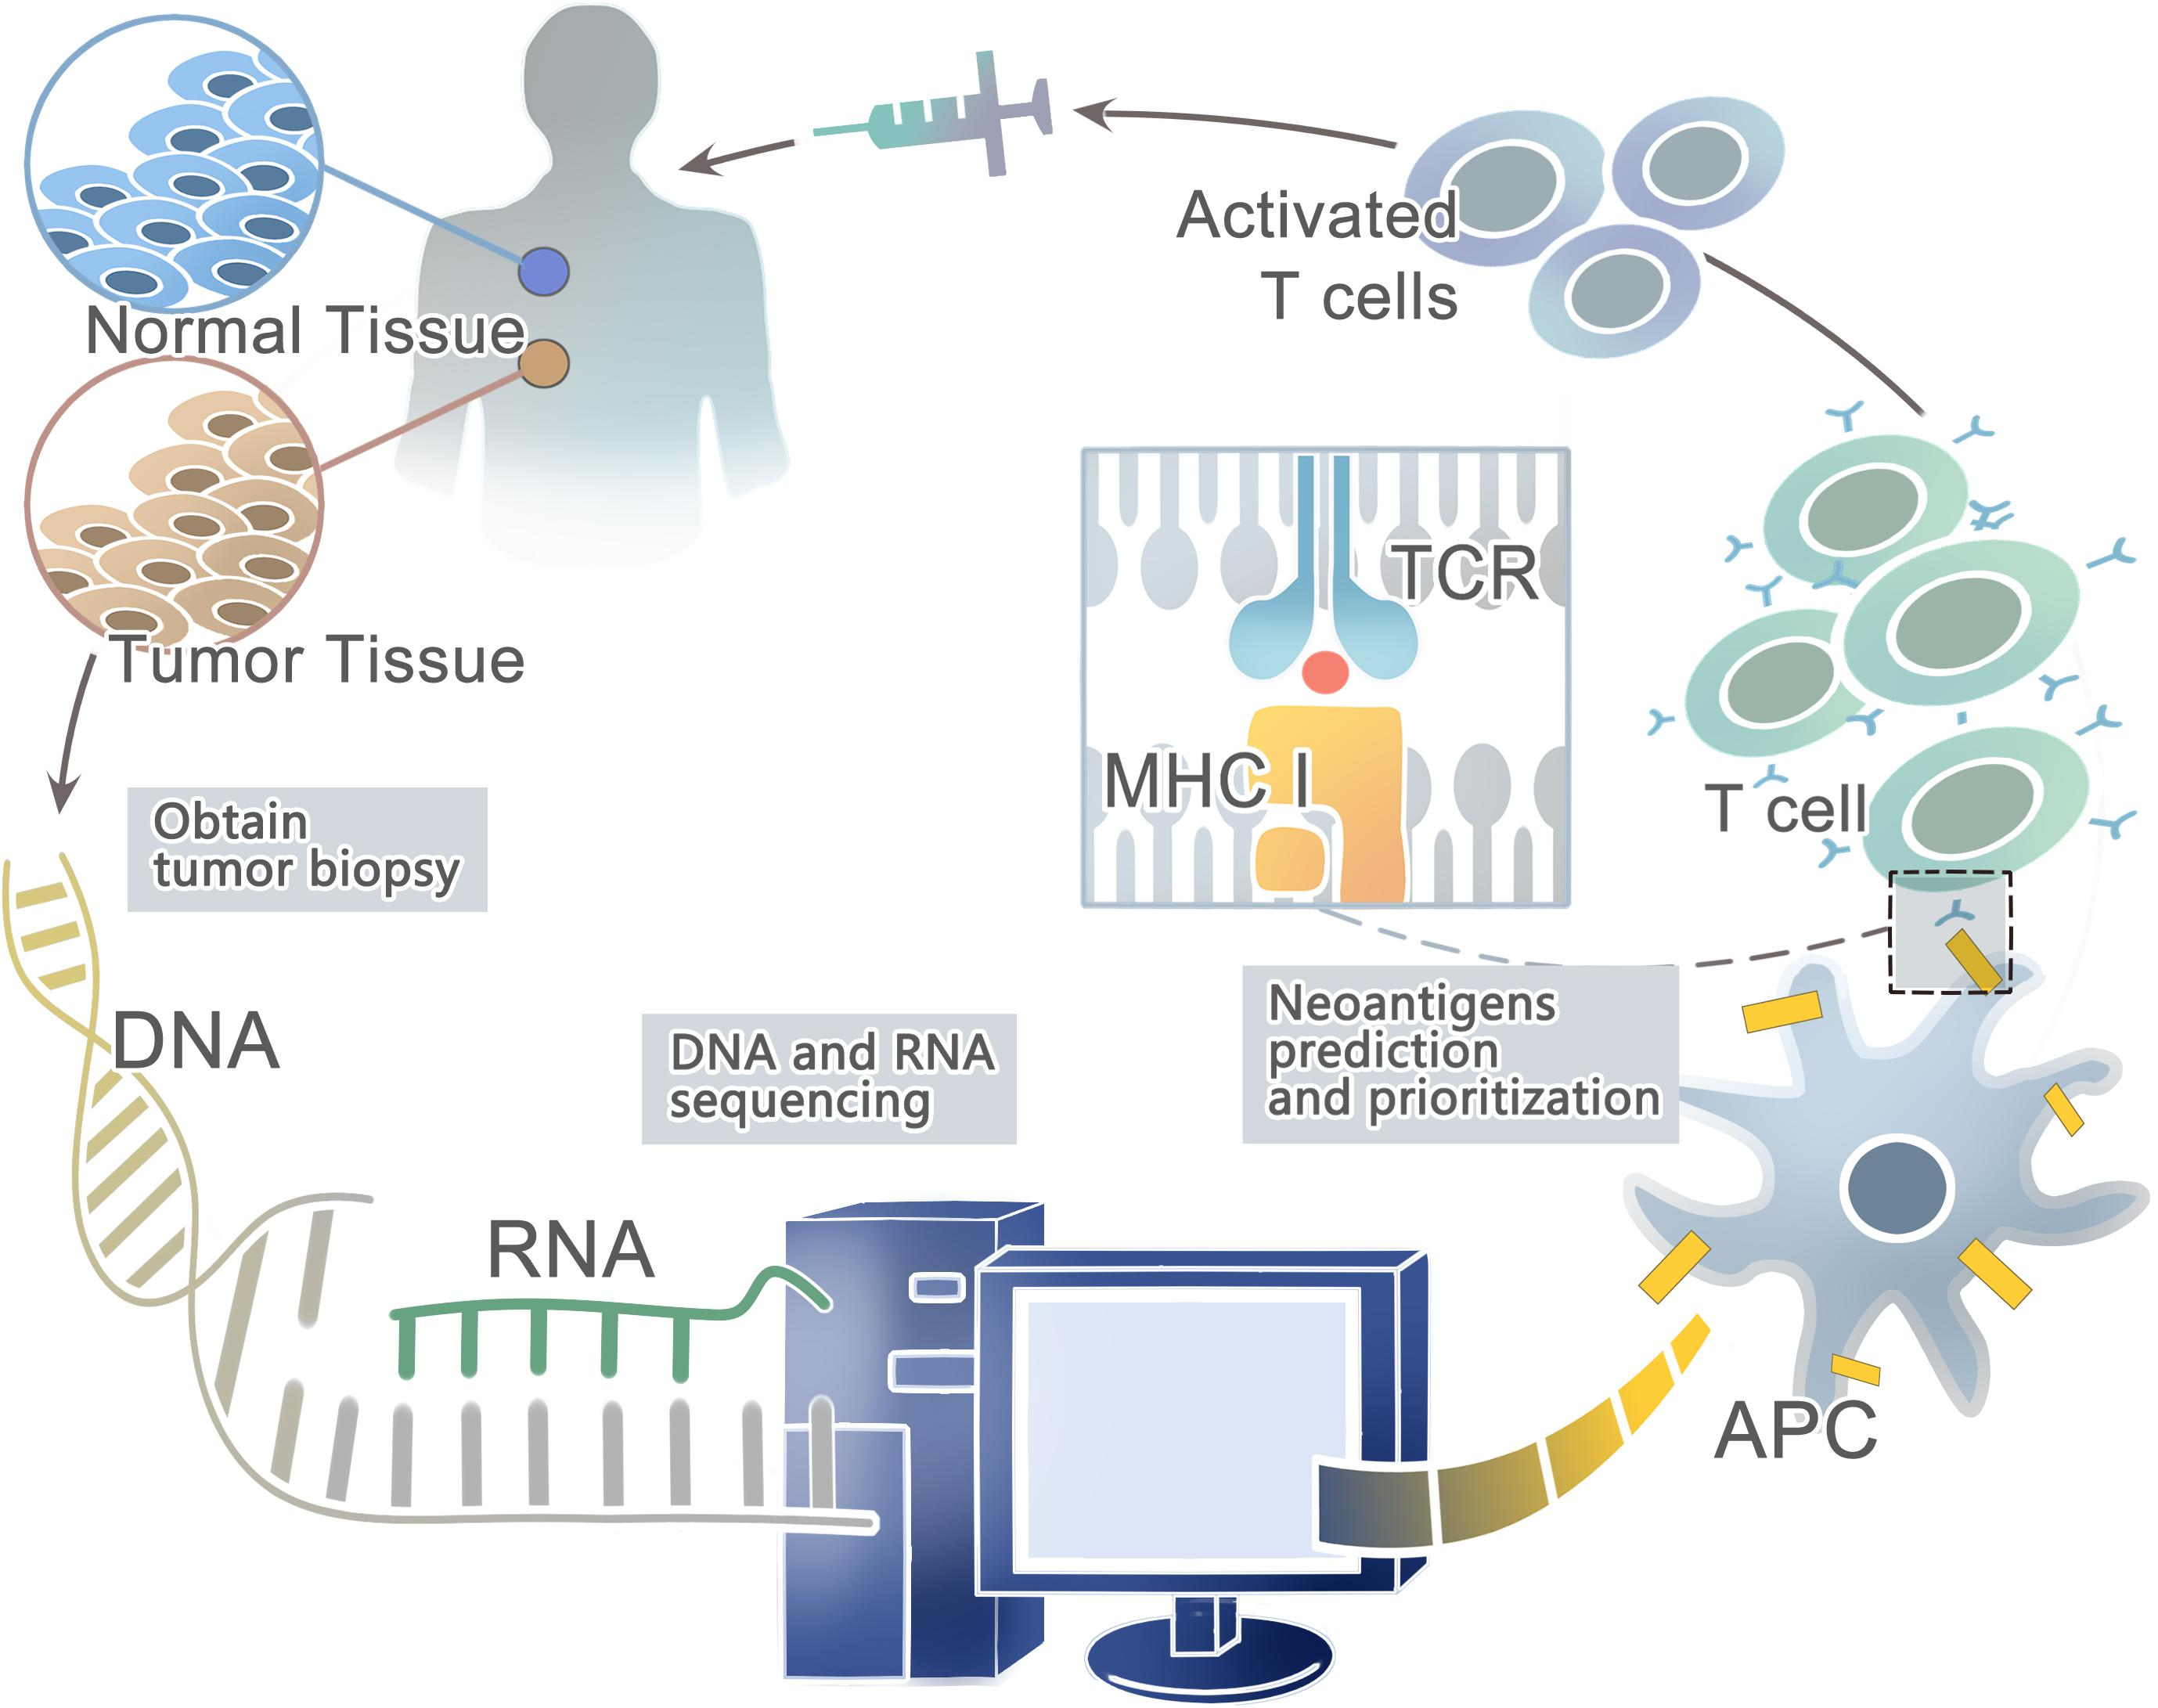
\includegraphics[width=\textwidth]{../img/vaccines/vaccine_pipeline}
		\caption{Proceso de desarrollo de vacunas.}
		\label{fig:vaccines_a}
	\end{subfigure}
	\hfill
	\begin{subfigure}[b]{0.44\textwidth}
		\centering
		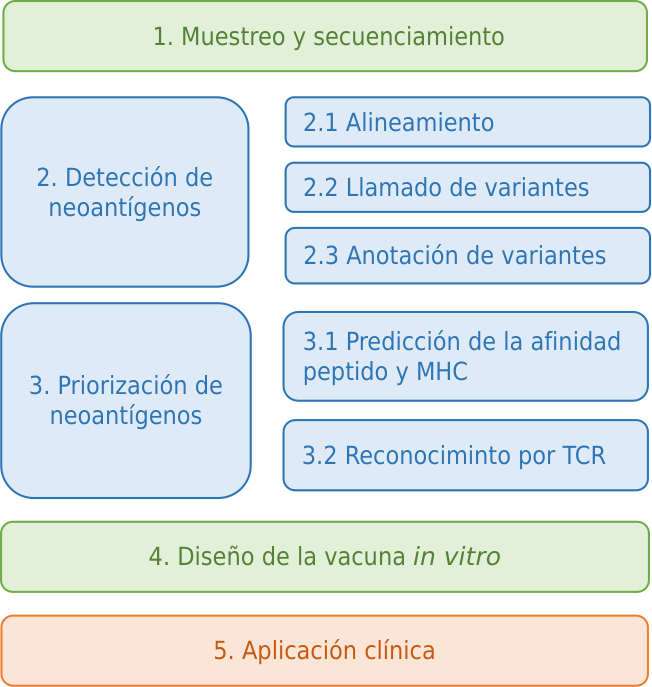
\includegraphics[width=\textwidth]{../img/vaccines/pipeline}
		\caption{\textit{Pipeline} para el desarrollo de vacunas.}
		\label{fig:vaccines_b}
	\end{subfigure}
	
	\caption{Marco de desarrollo para la elbaoración de vacunas personalizadas contra el cancer basadas en neoantígenos. (a) muestra un panorama general de cada etapa. (b) detalla cada fase enfatizando el desarrollo \textit{in-silico}.  Modificado de \cite{han2020progress}.}
	\label{fig:vaccines}
\end{figure}
	
	
La detección \textit{in-silico} de neoantígenos se basa en la segunda y tercera etapa de la Figura \ref{fig:vaccines_b}. En este contexto, debido a la complejidad del proceso y la cantidad de métodos existentes, se han desarrollado software y \textit{pipelines} para facilitar el uso de estas herramientas. En la Tabla \ref{tab:review_pipelines}, presentamos los \textit{pipelines} publicados a partir del 2018. Estos \textit{pipelines} utilizan diferentes tipos de información como entrada, así PGV Pipeline \citep{rubinsteyn2018computational} y PEPPRMINT \citep{zhou2023prioritizing} utilizan DNA-seq; sin embargo, otras herramientas como PGNneo \citep{tan2023pgnneo}, NAP-CNB \citep{wert2021predicting}, NaoANT-HILL \citep{coelho2020neoant}, ProGeo-neo \citep{li2020progeo}, ScanNeo \citep{wang2019scanneo} y Neopepse \citep{kim2018neopepsee} utilizan RNA-seq porque estas secuencias encapsulan mejor la información de mutaciones y \textit{non-coding regions} de ADN \citep{tan2023pgnneo}. \\

Con el objetivo de reducir la complejidad de los \textit{pipelines}, otras propuestas han optado por utilizar Variant Calling Files (VCF), como entrada. Estos archivos, contienen información de las mutaciones y son obtenidas a partir de métodos de alineamiento y llamado de mutaciones (etapas 2.1 y 2.2 de la Figura \ref{fig:vaccines_b}). De esta forma, herramientas como Valid-Neo \citep{terai2022valid}, HLA3D \citep{li2022hla3d}, Neoepiscope \citep{wood2020neoepiscope} , pVACtools \citep{hundal2020pvactools} y NeoPredPipe \citep{schenck2019neopredpipe}, reducen la cantidad de herramientas utilizadas en la deteccion de neoantígenos; sin embargo, los resultados obtenidos, pueden ser inferiores comparado con herramientas que usan DNA-seq y RNA-seq.\\

Adicionalmente, para una correcta detección de neoantígenos, es necesario contar con la secuenciación de proteínas Major Histocompatibility Complex (MHC) o Human Leukocyte Antigens (HLA). Es neceario contar con estas proteínas porque, son utilizadas para predecir la union entre posibles neoantígenos al MHC (pMHC: etapa 3.1 de la Figura \ref{fig:vaccines_b}). Estas proteínas son codificadas por genes altamente polimórficos, esto proporciona una variación sustancial en la unión de péptidos (neoantígenos), influyendo de esta manera en el conjunto de péptidos presentados a las células T. \citep{abualrous2021major}. En este contexto,  los \textit{pipelines} Valid-NEO \citep{terai2022valid}  y NeoPredPipe \citep{schenck2019neopredpipe} y Neopepsee \citep{kim2018neopepsee} solicitan como entrada estas proteínas; mientras que las otras predicen esta información a partir de DNA-seq.

% falta mencioan porque usan MS


	
\begin{table}[h]
	\caption{Lista de \textit{pipelines} desarrollados desde el 2018 hasta la actualidad para la detección de neoantígenos.}
	\label{tab:review_pipelines}
	\setlength{\tabcolsep}{0.5em} % for the horizontal padding
	{\renewcommand{\arraystretch}{1.5}% for the vertical padding
		
	
			\begin{tabular}{lp{0.6cm}p{3cm}p{4.5cm}p{2.7cm}}
	\textbf{Nombre} & \textbf{Año}  & \textbf{Ref.}                                 & \textbf{Entrada}                                         & \textbf{Salida}                                     \\ \hline
	
	PEPPRMINT         & 2023 &\cite{zhou2023prioritizing}         & DNA-seq                                                  & Neoantígenos                                        \\

	PGNneo & 2023	& \cite{tan2023pgnneo}	& VCF, RNA-seq y MS data	& Neoantígenos \\
	
	Valid-NEO       & 2022 &\cite{terai2022valid}             & VCF y HLA          & Neoantígenos  \\
	
	HLA3D & 2022	& \cite{li2022hla3d}	& VCF, HLA, SMG y HBV	& Neoantígenos \\
	
	
	
	NAP-CNB         & 2021 &\cite{wert2021predicting}         & RNA-seq                                                  & Neoantígenos                                       \\
	
	NeoANT-HILL     & 2020 &\cite{coelho2020neoant}           & RNA-seq y VCF                        & Neoantígenos y gene expression  \\
	
	Neoepiscope     & 2020 &\cite{wood2020neoepiscope}        & VCF y BAM                   & Neoantígenos y mutaciones                          \\
	
	ProGeo-neo      & 2020 &\cite{li2020progeo}               & RNA-seq y VCF                        & Neoantígenos                                       \\
	
	pVACtools       & 2020 &\cite{hundal2020pvactools}        & VCF                                         & Neoantígenos                                       \\
	
	NeoPredPipe     & 2019 &\cite{schenck2019neopredpipe}     & VCF y HLA                            & Neoantígenos y variant annotation              \\
	
	ScanNeo         & 2019 &\cite{wang2019scanneo}            & RNA-seq                                                  & Neoantígenos                                       \\
	
		
	Neopepsee       & 2018 &\cite{kim2018neopepsee}           & RNA-seq, VCF, HLA  & Neoantígenos y gene expression    \\ 
	
	PGV Pipeline    & 2018 &\cite{rubinsteyn2018computational}& DNA-seq                                                  & Neoantígenos                                       \\
	
	
	
	
	
\end{tabular}
	
	}
\end{table}




\section{Planteamiento del problema}

A pesar de varios esfuerzos en el desarrollo de \textit{pipelines} y algoritmos, menos del 5\% de neoantígenos detectados llegan a la membrana y activan el sistema immune \citep{de2020neoantigen, mill2022neoms, bulik2019deep, bassani2015mass, yadav2014predicting}. Según los autores de los \textit{pipelines} las razones pueden ser: (1) la no inclución de varias fuentes de información como DNA-seq, RNS-seq, y datos de \textit{Mass Spectrometry} (MS)  \citep{kim2018neopepsee}; (2) no considerar la etapa 3.2 de la Figura \ref{fig:vaccines_b} referente a un analisis para la predicción del pMHC al TCR \citep{rubinsteyn2018computational}; (3) y quizas la mas importante es no utilizar información de eventos de \textit{alternative splicing}, variaciones estructurales y la fusión de genes, esta información esta fuertemente relacionada con varios tipos de cancer \citep{wood2020neoepiscope}.

	
\section{Objetivos de la investigación}
	
	\subsection{Objetivo general}
	
	Desarrollar una aplicación Web para la detección de neoantígenos en el marco del desarrollo de vacunas personalizadas para tratar el Cáncer.
	
	\subsection{Objetivos específicos}
	\begin{enumerate}
		\item Implementar un método basado en \textit{transformers} y \textit{transfer learning} para predecir la unión pMHC.	
		\item Comparar los resultados del método propuesto con NetMHCpan4.1.
		\item Implementar la aplicación Web para la detección de neoantígenos.
	

		

		
	\end{enumerate}

	
\section{Importancia de la investigación}

El cáncer es el mayor problema de salud mundial; sin embargo, los métodos tradicionales basados en cirugías, radioterapias y quimioterapias tienen baja efectividad \citep{peng2019neoantigen}. En este contexto, los neoantígenos son factores clave en el desarrollo de vacunas contra el Cáncer  \citep{borden2022cancer,chen2021challenges,gopanenko2020main}. Si se logra desarrollar un método con un buen desempeño, la inmunoterapia del cáncer basada en el desarrollo de vacunas personalizadas, podría utilizarse como alternativa a otros métodos como radioterapias y quimioterapias. \\

En el área de la inteligencia artificial y específicamente en el tópico de \textit{deep learning}, el desarrollo de un método basado en \textit{transformers} y \textit{transfer learning}, representa una contribución importante  y demuestra que este tipo de modelos no solo pueden utilizarse en campos del procesamiento natural del lenguaje (como lo hace chatGPT) sino también en otros ámbitos como la Immunoinformática.\\

Finalmente, tener una aplicación Web desarrollada por la universidad La Salle, realza el nombre de la universidad y la iguala a otras universidades que también desarrollan aplicaciones basadas en inteligencia artificial para solucionar  problemas interdisciplinarios.


\section{Posibles soluciones y consecuencias de la investigación}

Entre las consecuencias de la investigación tenemos: (1) una publicación con el método propuesto para la predicción de la unión pMHC y (2) una aplicación Web para la predicción de la unión pMHC. Luego, esta investigación abre las puertas para futuros proyectos que involucren el desarrollo de un \textit{pipeline} para la detección de neoantígenos, pero esta vez tomando como entrada una secuencia de ADN. Otro futuro proyecto de mayor envergadura involucra un trabajo interdisciplinario con biotecnólogos, biólogos y oncólogos; con el objetivo de desarrollar vacunas personalizadas para tratar el Cáncer. 

\section{Diseño y secuencia lógica de la investigación} 

Hemos dividido la propuesta en dos partes: la primera se basa en el desarrollo de un modelo de \textit{deep learning} basado en \textit{transformers} y \textit{transfer learning} para la predicción de la unión pMHC. Actualmente, ya tenemos resultados preliminares con un desempeño comparable a NetMHCpan4.1 (\textit{state-of-art method}) \citep{arceda2023neoantigen} y adicionalmente, hemos desarrollado un \textit{review} sobre los principales métodos del estado del arte \citep{machaca2023deep}. En la segunda parte del proyecto, se propone desarrollar la aplicación Web para la detección de neoantígenos, enfocados en la predicción de la unión pMHC.

\subsection{Desarrollo del modelo de inteligencia artificial}

En este proyecto, se propone utilizar una arquitectura BERT con \textit{transfer learning}. Analizamos alternativas como TAPE \citep{rao2019evaluating}, ProtBERT-BFD \citep{elnaggar2021prottrans}, ESM-1b \citep{rives2021biological} y ESM2 \citep{lin2023evolutionary} cada una con 92 millones, 420 millones, 650 millones y 15 billones de parámetros respectivamente. TAPE fue entrenado con 30 millones de proteínas, ProtBERT-BFD con 2122 millones de proteínas y 250 millones de proteínas para ESM-1b. Además, ESM-1b obtuvo mejores resultados en precisión de contacto que TAPE y ProtBERT-BFD \citep{rives2021biological}; sin embargo, ya contamos la versión nueva ESM2 \citep{lin2023evolutionary}.\\

Además, HLAB \citep{zhang2022hlab} propuso el uso de ProtBERT-BFD \citep{elnaggar2021prottrans} con un modelo BiLSTM en cascada y superó a NetMHCpan4.1 (método de vanguardia) en el \textit{allele} HLA-A*01:01. Por lo tanto, en este proyecto, proponemos utilizar el modelo preentrenado ESM2 \citep{lin2023evolutionary} con un capa BiLSTM  similar a HLAB \citep{zhang2022hlab}. Para el \textit{fine-tuning}, utilizaremos conjuntos de datos de NetMHCpan4.1 y NetMHCIIpan4.0.\\

En resumen, en la Figura. \ref{fig:proposal}, presentamos la propuesta: primero, se concatenan y se aplica \textit{padding} al péptido y la pseudo secuencia MHC; en segundo lugar, utilizamos el modelo \textit{transformer} ESM2 para obtener una nueva representación de los aminoácidos; finalmente, utilizamos un BiLSTM para predecir el enlace pMHC. 





\begin{figure}[H]
	\centering
	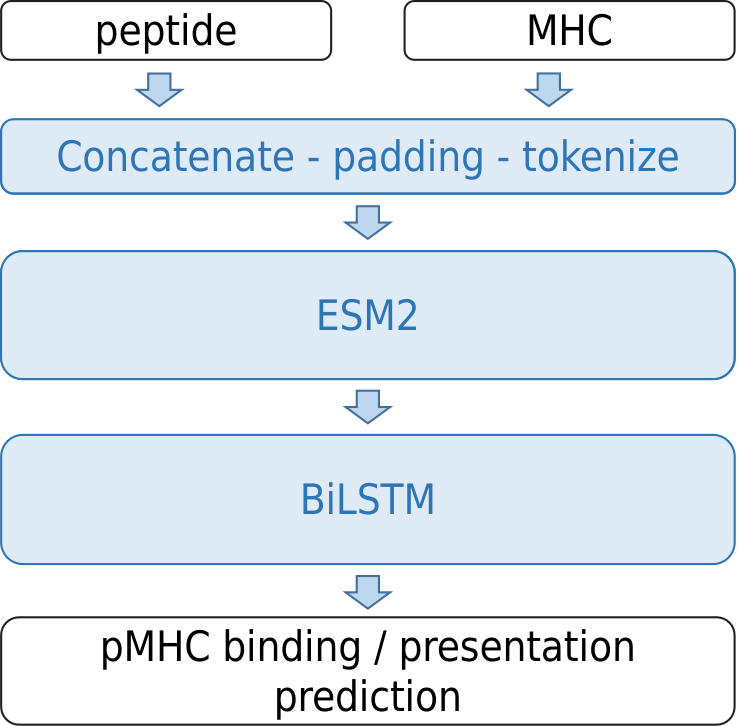
\includegraphics[width=0.35\textwidth]{../img/neoantigen/proposal1}
	\caption{Propuesta: Utilizamos el modelo de transformer ESM2 seguido de BiLSTM para predecir el enlace pMHC.}
	\label{fig:proposal}
\end{figure}

\subsection{Desarrollo de la aplicación Web}

La aplicación Web se desarrollará para que un usuario pueda realizar predicciones de la unión pMHC. La página Web tomará como entrada un conjunto de péptidos y un tipo de MHC. Luego, retornará y mostrará que péptidos pueden unirse a dicho MHC y por lo tanto se les considera posibles neoantígenos.\\

Referente a las tecnologías a utilizar: para el \textit{BackEnd}, se utilizará el \textit{framework} Express.js de Javascript y el gestor de base de datos Mongo. Para el \textit{FrontEnd}, se propone utilizar Next.js. Se han seleccionado estas tecnologías debido a su versatilidad y la enorme documentación que presentan. La Figura \ref{fig:arquitectura} anterior, muestra el nodo del FrontEnd donde se tiene la interfaz de un navegador web responsivo, consumiendo el servicio disponible desde el BackEnd. En la implementación la aplicación web en NodeJS Express y la base de datos Mongo se encuentran en el mismo servidor.


\begin{figure}[H]
	\centering
	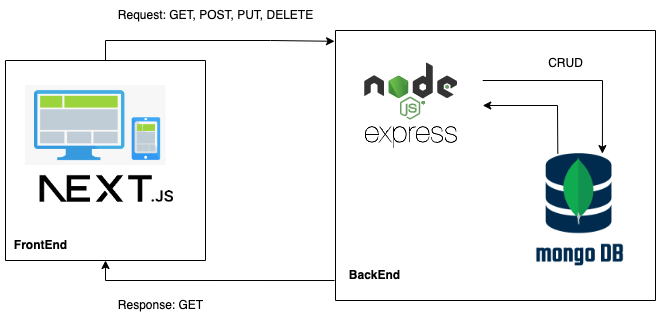
\includegraphics[width=0.8\textwidth]{../img/neoantigen/arquitectura.png}
	\caption{Arquitectura de la aplicación Web.}
	\label{fig:arquitectura}
\end{figure}


	
	\bibliographystyle{apalike}
	\bibliography{../bibliography}

\clearpage


%%%%%%%%%%%%%%%%%%%%%%%%%%%%%%%%%%%%%%%%%%%%%%%%%%%%%%%%%%%%%%%%%%%%%%
%%%%%%%%%%%%%%%%%%%%%%%%%%%%%%%%%%%%%%%%%%%%%%%%%%%%%%%%%%%%%%%%%%%%%%
%%%%%%%%%%%%%%%%%%%%%%%%%%%%%%%%%%%%%%%%%%%%%%%%%%%%%%%%%%%%%%%%%%%%%%
%%%%%%%%%%%%%%%%%%%%%%%%%%%%%%%%%%%%%%%%%%%%%%%%%%%%%%%%%%%%%%%%%%%%%%
\part*{Gestión del Proyecto}

\setcounter{section}{0}
%%%%%%%%%%%%%%%%%%%%%%%%%%%%%%%%%%%%%%%%%%%%%%%%%%%%%%%%%%%%%%%%%%%%%%
%%%%%%%%%%%%%%%%%%%%%%%%%%%%%%%%%%%%%%%%%%%%%%%%%%%%%%%%%%%%%%%%%%%%%%
%%%%%%%%%%%%%%%%%%%%%%%%%%%%%%%%%%%%%%%%%%%%%%%%%%%%%%%%%%%%%%%%%%%%%%


\section{Integrantes del equipo}
En la Tabla \ref{tab:integrantes}, presentamos al equipo de investigación.

\begin{table}[H]
\caption{Integrantes del equipo de investigación}
\label{tab:integrantes}
\setlength{\tabcolsep}{0.5em} % for the horizontal padding
{\renewcommand{\arraystretch}{1.2}% for the vertical padding
\begin{tabular}{|p{3cm}p{2.2cm}p{2.3cm}p{2.5cm}p{3.3cm}|} \hline
\textbf{Nombre y apellidos} & \textbf{Cargo}         & \textbf{Escuela profesional} & \textbf{Rol del proyecto} & \textbf{Descripción breve del rol} \\ \hline
Vicente Machaca Arceda      & Investigador principal & Ingeniería de Software       & Investigador principal    & Investigación y desarrollo         \\
Richart Escobedo Quispe     & Co-investigador        & Ingeniería de Software       & Co-investigador           & Investigación y desarrollo         \\
Estudiante 01               & Asistente              & Ingeniería de Software       & Asistente                 & Desarrollo                         \\
Estudiante 02               & Asistente              & Ingeniería de Software       & Asistente                 & Desarrollo          \\ \hline              
\end{tabular}
}
\end{table}


\section{Presupuesto y cronograma}

En la Tabla \ref{tab:presupuesto}, presentamos el presupuesto para el trabajo de investigación. Este asciende a la suma de 4000 mil soles.

\begin{table}[H]
	\centering
	\setlength{\tabcolsep}{0.5em} % for the horizontal padding
	{\renewcommand{\arraystretch}{1.2}% for the vertical padding
		\caption{Presupuesto. Abreviaciones, PC: \textit{Personal Computer}}
		\label{tab:presupuesto}
		\begin{tabular}{|p{1.5cm}|p{8.2cm}|c|c|c|} \hline
			\textbf{Incentivo}    & \textbf{Miembro del equipo}    & \textbf{Unidades} & \textbf{Precio} & \textbf{Total} \\ \hline
			Incentivos & Incentivo al investigador principal          & 1                 & 700            & 700           \\
			& Incentivo al co-investigador & 1                 & 700            & 700           \\ \hline \hline
			
			\textbf{Hito}    & \textbf{Insumo o material}    & \textbf{Unidades} & \textbf{Precio} & \textbf{Total} \\ \hline
			Hito I & Workshops y cursos       & 2                 & 500            & 1000           \\
			& Servicios de \textit{cloud computing} para entrenar los modelos       & 1                 & 1000            & 1000           \\ \hline
			Hito II &  Hosting y dominio                      & 1                 & 600            & 600           \\
			 \hline
			& \textbf{Total}                         &                   &                 & \textbf{4000}         \\ \hline
		\end{tabular}
	}
\end{table}


En la Tabla \ref{tab:actv}, presentamos el cronograma de actividades por mes. IA: Inteligencia Artificial.

\begin{table}[H]
	\centering
	\setlength{\tabcolsep}{0.5em} % for the horizontal padding
	{\renewcommand{\arraystretch}{1.2}% for the vertical padding
		\caption{Cronograma de actividades por mes.}
		\label{tab:actv}
	\begin{tabular}{|p{5.5cm}|p{4cm}|c|c|c|c|c|c|c|} \hline
		\textbf{Actividades}                                  &   \textbf{Entregable}         & I & II & III & IV & V & VI & VII  \\ \hline
		
		\textbf{HITO I} &  Código fuente del modelo & & & & & & & \\
		Revisión de la literatura       &                       & x                     & x                      & x                       & x                      &                       &                        &                                                  \\
		Implementación del modelo de IA  &                           &       x                &           x             &                x         & x                      &                       &                        &                                                \\
		Evaluación y comparación del modelo &    &                       &                        & x                       & x                      & x                     &                        &                                                   \\
		
		\textbf{HITO II} & Página Web & & & & & & & \\
		Implementación de la página Web &  &                     &                        &                         & x                      & x                     & x                      &                                                  \\
		Redacción del artículo de investigación  &                                      &                       &                        &                         &                        & x                     & x                      & x                                              \\
		Difusión de resultados    &                              &                       &                        &                         &                       &                      &                       & x                                             \\ \hline
	\end{tabular}
}
\end{table}

\section{Propuesta de la conferencia o revista}

El artículo de investigación será presentado a la conferencia: ``18th International Conference on Practical Applications of Computational Biology \& Bioinformatics'' (\href{https://www.pacbb.net/}{enlace}). Está conferencia indexa los artículos en Scopus a tambien en la revista Lecture Notes in Networks and Systems que es H-index 27 según Scimago (\href{https://www.scimagojr.com/journalsearch.php?q=21100901469&tip=sid&clean=0}{enlace}). A su vez, está conferencia invita a los mejores artículos a una publicación extendida en revistas \textit{Quartil Q1}.


\section{Enlaces web de los CV de los miembros del grupo }

En la Table \ref{tab:inve}, presentamos los enlaces a los CV's del CTI vitae y el código RENACYT.

\begin{table}[H]
\centering
\caption{CV de los investigadores.}
\label{tab:inve}
\setlength{\tabcolsep}{0.5em} % for the horizontal padding
{\renewcommand{\arraystretch}{1.2}% for the vertical padding
\begin{tabular}{|lll|} \hline
\textbf{Nombre y apellidos} & \textbf{Link CTI vitae}                                                                      & \textbf{Código RENACYT} \\ \hline
Vicente Machaca Arceda      & \href{https://dina.concytec.gob.pe/appDirectorioCTI/VerDatosInvestigador.do?id\_investigador=22551}{enlace} & P0022551                \\
Richart Escobedo Quispe     & \href{https://dina.concytec.gob.pe/appDirectorioCTI/VerDatosInvestigador.do?id\_investigador=20597}{enlace} & -     \\ \hline                 
\end{tabular}
}
\end{table}


	
\end{document}